\item[(g)]
\section{FIR Filter Design with Hamming Window}

\subsection*{Problem Statement}
Now, use a Hamming window instead of the rectangular window (for \( N = 90 \)) and assess the result.

\subsection*{Theoretical Background}
The Hamming window is another window function used to design FIR filters. It has a better frequency response than the rectangular window, as it reduces the side lobes in the frequency domain, leading to less ripple in the stopband. The Hamming window is defined as:
\[ w[n] = 0.54 - 0.46 \cos \left( \frac{2\pi n}{N-1} \right) \]

\subsection*{Mathematical Derivation}
\begin{enumerate}
    \item Compute the ideal impulse response \( h_{\text{ideal}}[n] \) for \( N = 90 \).
    \item Apply the Hamming window to the ideal impulse response to obtain the windowed impulse response.
    \item Compute the frequency response of the windowed impulse response.
\end{enumerate}

\subsection*{Implementation and Results}
The frequency response of the FIR filter with a Hamming window for \( N = 90 \) is computed and plotted using Python. The plot below illustrates the frequency response along with the specified tolerance scheme.

\begin{figure}[h]
    \centering
    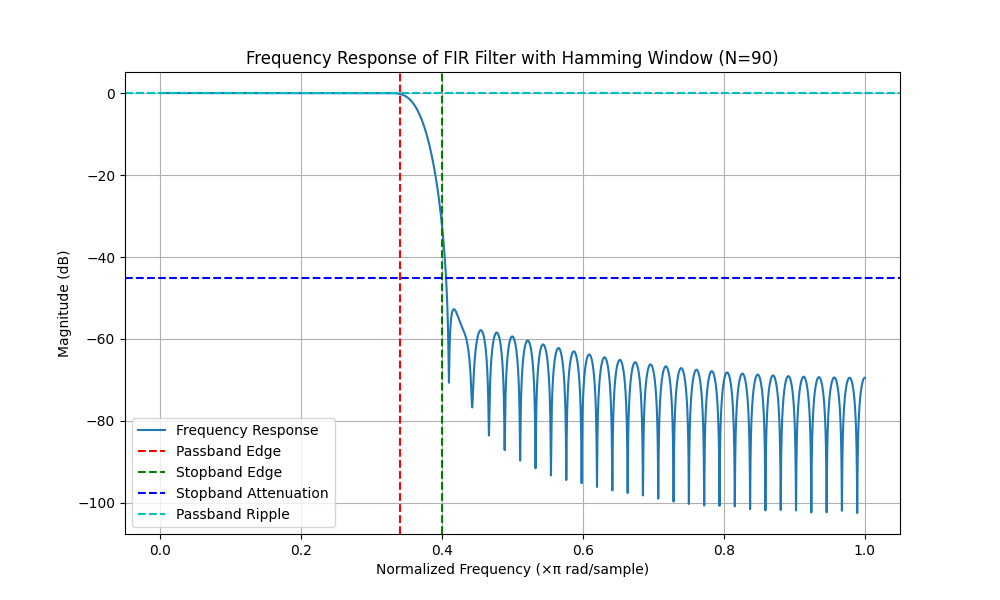
\includegraphics[width=0.8\textwidth]{fig/ex4_g_frequency_response_hamming.png}
    \caption{Frequency Response of FIR Filter with Hamming Window (N=90)}
    \label{fig:ex4_g_frequency_response_hamming}
\end{figure}

\subsection*{Conclusion}
The frequency response plot shows the performance of the FIR filter designed with a Hamming window of order \( N = 90 \). The Hamming window provides a better frequency response compared to the rectangular window, with reduced ripple in the stopband and a sharper transition band.
